\documentclass[11pt]{article}

%%%%%% better plots

\usepackage{adjustbox} % for size



% TITLE , but needs to be 'made' (see below)

\title{My first replicable Paper}
\author{
        MyFirstName MyLastName\\
        Evans School of Public Policy and Governance\\
        University of Washington\\
        Seattle, WA 98115, \underline{United States}\\
        \texttt{greatguy@uw.edu}
}
\date{\today}


% notice \begin...\end
\usepackage{Sweave}
\begin{document}
\Sconcordance{concordance:PaperInR_4.tex:PaperInR_4.Rnw:%
1 22 1 1 0 33 1 1 7 5 1 1 4 9 1 2 2 13 1 1 2 10 0 1 2 5 1 2 2 18 1 2 2 %
16 1 2 2 10 1}


\maketitle % this will use the previous information. Do NOT MOVE.

% an abstract, notice \begin...\end

\begin{abstract}
This is an example on how to make a reproducible paper. We are using R from Rstudio, creating an RSweave document. This is a nice start to create a nice paper and get an A+. The next sections will show the steps taken.
\end{abstract}

% a section, notice it has a label for easy 'referencing'
\section{Introduction}\label{intro}  %if no number is needed \section*

This is my intro to my great paper, I will explain the cool things I can do with my new `computational thinking' powers combined with some Latex. This is my intro to my great paper, I will explain the cool things I can do with my new `computational thinking' powers combined with some Latex. This is my intro to my great paper, I will explain the cool things I can do with my new `computational thinking' powers combined with some Latex. This is my intro to my great paper, I will explain the cool things I can do with my new `computational thinking' powers combined with some Latex.

% the newlines are not read:
This is my nice intro to my great paper, 
I will explain the cool things 
I can do with my new `computational thinking' 
powers
combined with some Latex.


\section{Exploring Data}\label{explo}

% footnotes, italic with \emph and referencing:
Sections may use a label\footnote{In fact, you can have a label wherever you think a future reference to that content might be needed.}. This label is needed for referencing. For example the next section has label \emph{datas}, so you can reference it by writing: As we see in section \ref{catexplo}.


%%%%%% code for loading here




\subsection{Exploring Categorical Data}\label{catexplo}

Here, I continue doing this nice work, I hope you like it and read it. It has been a very hard work.Here, I continue doing this nice work, I hope you like it and read it. It has been a very hard work.Here, I continue doing this nice work, I hope you like it and read it. It has been a very hard work.Here, I continue doing this nice work, I hope you like it and read it. It has been a very hard work.Here, I continue doing this nice work, I hope you like it and read it. It has been a very hard work.Here, I continue doing this nice work, I hope you like it and read it. It has been a very hard work.Here, I continue doing this nice work, I hope you like it and read it. It has been a very hard work.Here, I continue doing this nice work, I hope you like it and read it. It has been a very hard work.Here, I continue doing this nice work, I hope you like it and read it. It has been a very hard work.

%%%%%% code for exploring here

%%%%%%

You can see this variable plotted in Figure \ref{catexplore_plot}

\begin{figure}[h]
\centering
\begin{adjustbox}{width=7cm,height=5cm}
%\begin{adjustbox}{width=7cm,height=5cm,clip,trim=0cm 2cm 0cm 0cm} 
%trimmimg: left,bottom, right,top
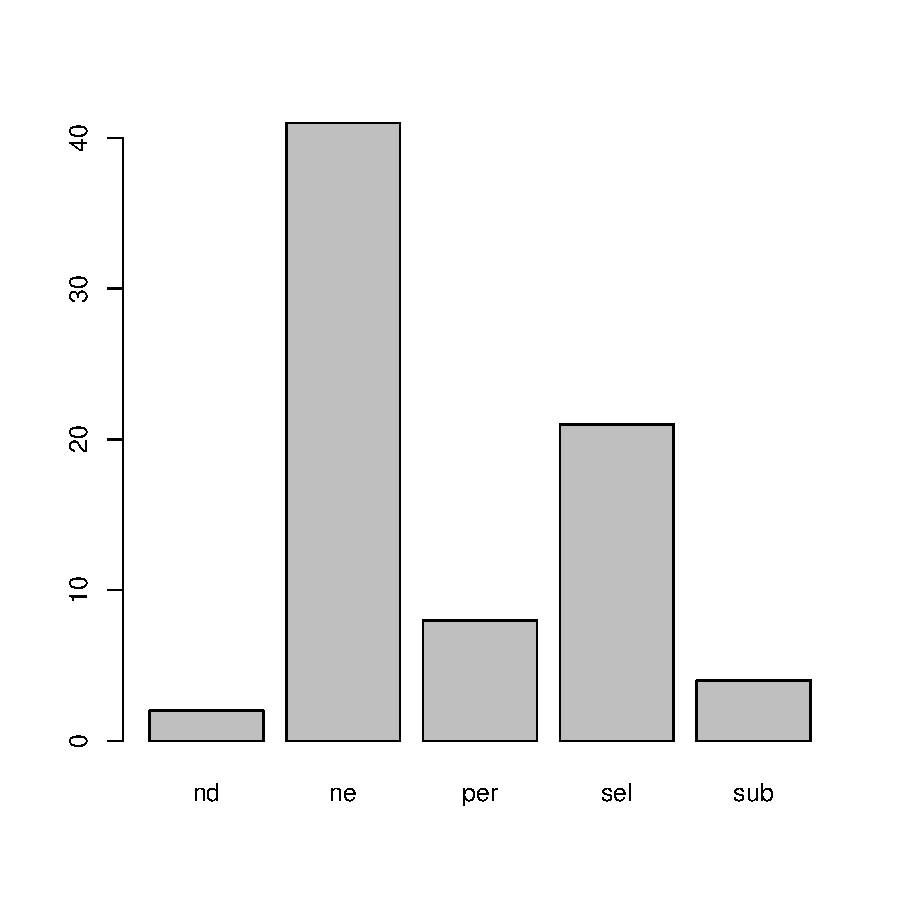
\includegraphics{PaperInR_4-cat_plot}
\end{adjustbox}
\caption{ONI barplot}  %title
\label{catexplore_plot} % for \ref{}
\end{figure}





\subsection{Exploring Numerical Data}\label{numexplo}

Here, I continue doing this nice work, I hope you like it and read it. It has been a very hard work.Here, I continue doing this nice work, I hope you like it and read it. It has been a very hard work.Here, I continue doing this nice work, I hope you like it and read it. It has been a very hard work.Here, I continue doing this nice work, I hope you like it and read it. It has been a very hard work.Here, I continue doing this nice work, I hope you like it and read it. It has been a very hard work.Here, I continue doing this nice work, I hope you like it and read it. It has been a very hard work.Here, I continue doing this nice work, I hope you like it and read it. It has been a very hard work.Here, I continue doing this nice work, I hope you like it and read it. It has been a very hard work.Here, I continue doing this nice work, I hope you like it and read it. It has been a very hard work.

%%%%%% code for exploring here
\begin{Schunk}
\begin{Soutput}
       FH             RWB       
 Min.   :10.00   Min.   : 6.38  
 1st Qu.:43.50   1st Qu.:28.22  
 Median :61.00   Median :37.99  
 Mean   :58.91   Mean   :39.67  
 3rd Qu.:80.00   3rd Qu.:46.85  
 Max.   :97.00   Max.   :83.90  
\end{Soutput}
\end{Schunk}



\begin{figure}[h]
\centering
\begin{adjustbox}{width=7cm,height=5.5cm,clip,trim=0cm 1cm 0cm 0cm} 
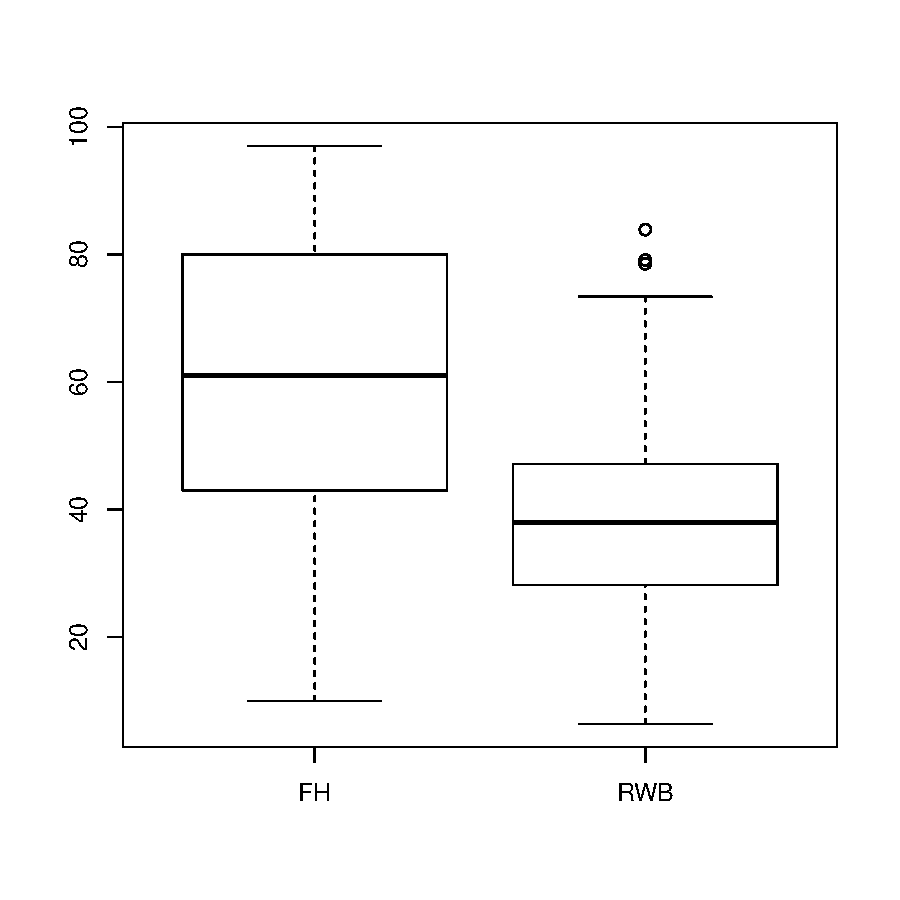
\includegraphics{PaperInR_4-num_plot}
\end{adjustbox}
\caption{boxplots}  %title
\label{num_plot} % for \ref{}
\end{figure}


Boxplots were introduced by Tuckey (Tukey, John W (1977). Exploratory Data Analysis. Addison-Wesley.)

\section{Looking for Relationships}\label{bivar}


Here, I continue doing this nice work, I hope you like it and read it. It has been a very hard work.Here, I continue doing this nice work, I hope you like it and read it. It has been a very hard work.Here, I continue doing this nice work, I hope you like it and read it. It has been a very hard work.Here, I continue doing this nice work, I hope you like it and read it. It has been a very hard work.Here, I continue doing this nice work, I hope you like it and read it. It has been a very hard work.Here, I continue doing this nice work, I hope you like it and read it. It has been a very hard work.Here, I continue doing this nice work, I hope you like it and read it. It has been a very hard work.Here, I continue doing this nice work, I hope you like it and read it. It has been a very hard work.Here, I continue doing this nice work, I hope you like it and read it. It has been a very hard work.

\subsection{Numerical and  Categorical}\label{binumcat}


\begin{figure}[h]
\centering
\begin{adjustbox}{width=7cm,height=7cm,clip,trim=0cm 0cm 0cm 0cm} 
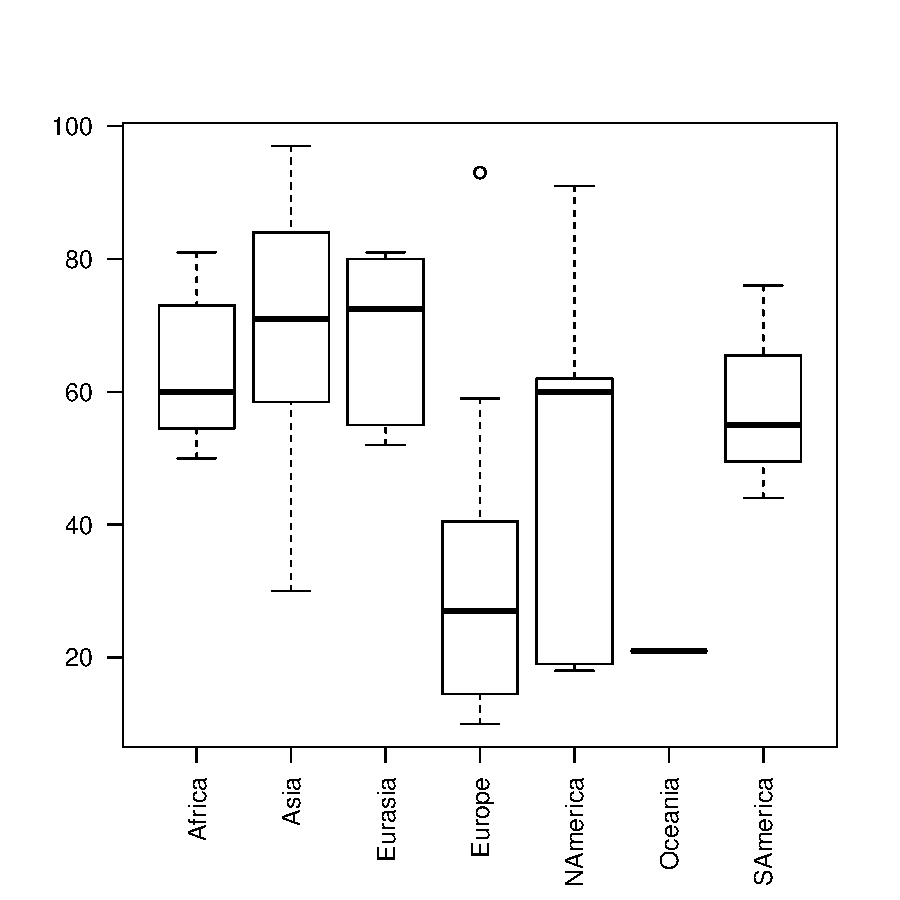
\includegraphics{PaperInR_4-numcat_plot}
\end{adjustbox}
\caption{boxplots}  %title
\label{numcat_plot} % for \ref{}
\end{figure}


Here, I continue doing this nice work, I hope you like it and read it. It has been a very hard work.Here, I continue doing this nice work, I hope you like it and read it. It has been a very hard work.Here, I continue doing this nice work, I hope you like it and read it. It has been a very hard work.Here, I continue doing this nice work, I hope you like it and read it. It has been a very hard work.Here, I continue doing this nice work, I hope you like it and read it. It has been a very hard work.Here, I continue doing this nice work, I hope you like it and read it. It has been a very hard work.Here, I continue doing this nice work, I hope you like it and read it. It has been a very hard work.Here, I continue doing this nice work, I hope you like it and read it. It has been a very hard work.Here, I continue doing this nice work, I hope you like it and read it. It has been a very hard work.

\subsection{Numerical and Numerical}\label{binumnum}

Here, I continue doing this nice work, I hope you like it and read it. It has been a very hard work.Here, I continue doing this nice work, I hope you like it and read it. It has been a very hard work.Here, I continue doing this nice work, I hope you like it and read it. It has been a very hard work.Here, I continue doing this nice work, I hope you like it and read it. It has been a very hard work.Here, I continue doing this nice work, I hope you like it and read it. It has been a very hard work.Here, I continue doing this nice work, I hope you like it and read it. It has been a very hard work.Here, I continue doing this nice work, I hope you like it and read it. It has been a very hard work.Here, I continue doing this nice work, I hope you like it and read it. It has been a very hard work.Here, I continue doing this nice work, I hope you like it and read it. It has been a very hard work.
%%%%%% code for exploring here


\begin{figure}[h]
\centering
\begin{adjustbox}{width=7cm,height=5.5cm,clip,trim=0cm 1cm 0cm 0cm} 
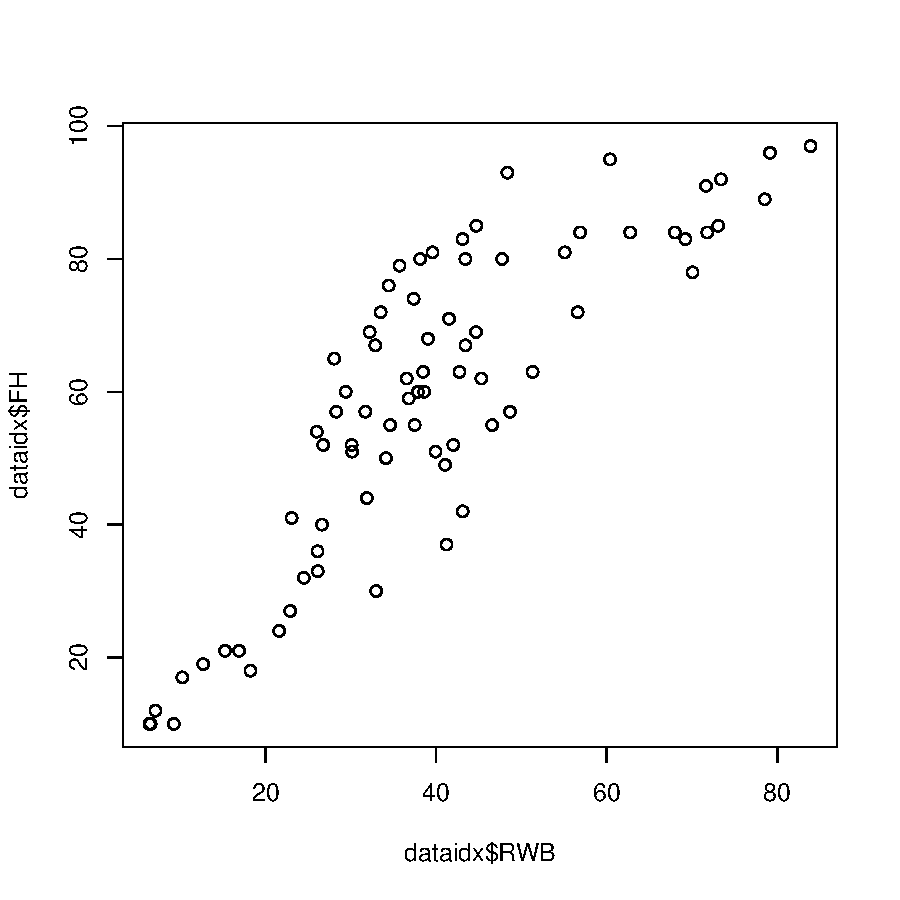
\includegraphics{PaperInR_4-numnum_plot}
\end{adjustbox}
\caption{boxplots}  %title
\label{numnum_plot} % for \ref{}
\end{figure}


The scatter plot is thought to be invented by  John Frederick W. Herschel according to this link: https://qz.com/1235712/the-origins-of-the-scatter-plot-data-visualizations-greatest-invention/



\end{document}
